\section{Introduction}

Planning means accepting a worse result now for a better one later. A chess player gives up a pawn to open a file. A card player spends a turn weakening an opponent before attacking. Language models now act as agents that are expected to plan in this sense. Their instructions often say so directly: think ahead, consider the long run, optimize over the next several steps. Whether a model actually changes its decision when told to look further ahead is a basic question. Current benchmarks cannot answer it.

The difficulty is that the horizon is rarely the only thing that changes. Planning benchmarks pose problems whose length varies together with their content \citep{valmeekam2023planbench,zheng2024naturalplan,xie2024travelplanner}. Game benchmarks score a whole episode, which mixes rule knowledge, tactics and luck into one number \citep{costarelli2024gamebench,paglieri2025balrog,park2025orak}. When a model does worse on a longer task, we cannot tell whether it failed to look ahead or whether the longer task was simply harder. A clean answer needs the same problem posed twice, with only the horizon changed, and a ground truth for each version.

This paper provides that test. Each item is one frozen state from a deterministic, turn-based card game. We ask a model for its next move under a goal measured after $H$ decisions, for $H \in \{1,2,4,8\}$. Everything else stays identical: the state, the legal moves, the scoring rule and the answer format. Exhaustive search over the game's simulator gives the exact value of every legal move at every horizon. Figure~\ref{fig:example} shows a state from the test. A quick attack wins if the goal is one decision away. A setup move that makes every later hit land harder wins if the goal is eight decisions away.

Two design choices make the test hard to fool. First, a model that ignores the horizon scores exactly zero on our main measure. We judge its long-horizon and short-horizon answers by the same long-horizon standard, so only a changed answer can earn credit. Second, half of the states are controls, where the best move is the same at every horizon. A model that merely reacts to a longer instruction moves its answers on both kinds of state. A model that uses the horizon moves them only where the horizon matters.

We chose a card game because it is a rare domain where all of this is possible at once. Short-term and long-term moves come apart naturally. The full state fits in about a thousand tokens of text. A simulator can be copied and searched exactly. The game is also an established testbed for language agents \citep{bateni2024language,park2025orak}.

We test eight open-weight models from four families. Three findings stand out.
\begin{itemize}
\item \textbf{Only large reasoning models respond to the horizon.} Qwen3-32B and gpt-oss-120b choose the long-horizon move more often when told to look eight decisions ahead. Smaller models and models without explicit reasoning do not, including a 70-billion-parameter model.
\item \textbf{Responding is not planning.} The responsive models give up the greedy move, but only about one time in three do they replace it with the correct long-horizon move. On control states they also abandon moves that were already right, so their scores do not improve.
\item \textbf{The pattern is not about knowing the game.} A pre-registered test that supplies an exact rulebook leaves the picture unchanged, and so does a second test that replaces every card and enemy name with a code.
\end{itemize}

We make three contributions. The first is a controlled-horizon benchmark of 1,760 game states with an exact answer key at four horizons. The second is a protocol for building such benchmarks in any domain with a simulator, including scoring that a model cannot game by ignoring the instruction. The third is evidence that current models treat ``look further ahead'' as a cue to avoid the obvious answer, without optimizing for the horizon they were given. All analyses were frozen before the models ran, and every amendment is versioned. We release the states, the exact action values, the prompts and every model response.

\begin{figure}[t]
\centering
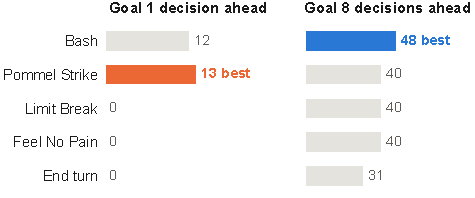
\includegraphics[width=\columnwidth]{figures/example.pdf}
\caption{One state from the benchmark (Ironclad against the Slime Boss, 2 energy). The boss is \emph{Vulnerable}, taking 50\% more damage, for one more turn. Bars give the exact value of each legal move, found by exhaustive search. With a one-decision goal, Pommel Strike deals the most damage now. With an eight-decision goal, Bash is best. It deals slightly less now but extends Vulnerable, so the attacks of the next turns keep their bonus. The state, the moves and the scoring rule are identical in both prompts. Only $H$ changes.}
\label{fig:example}
\end{figure}
